\documentclass[letterpaper,12pt]{article}   %%% Can be report

%% set paper margins
\oddsidemargin=0.1in
\evensidemargin=0.1in
\textwidth=6.0in
\topmargin=-0.7in
\textheight=9.0in
\parindent=0.2in

\usepackage{amsmath,amssymb,bm}
\usepackage{graphicx}
\usepackage{rotating}
\usepackage{subfigure}
\graphicspath{%
  {figs/ipe/}
  {figs/dia/}
  {figs/matlab/}
} 
\usepackage[width=11cm,font=footnotesize,labelfont=bf, %
format=default,justification=centerlast]{caption} % Figure caption text customization 

\usepackage{pgfgantt}


\usepackage{hyperref}
\usepackage{soul}
\usepackage{setspace}
\usepackage{multirow}

\usepackage{siunitx}
\sisetup{unitsep=\cdot}

\title{ECE498:~Senior Capstone Project I\\\textbf{\underline{Project Proposal}}\\
\vspace{0.5in}
Project Title: BEMOSS}
\vspace{1.5in}
\author{Reece Bachman Robert O'Malley and Jordan Ingram\\ Advisor: Dr.~Suruz Miah
}
%\date{February 6, 2003}  No need to write, Date will be automatically on the title page
\date{}  % Do not show date on the title page

%%%%%%%%%%%%%%%%% Set document line spacing %%%%%%%%%%%%%%%%%%%%%
\singlespacing
%\onehalfspacing
%\doublespacing
% all packages are in the following tex file.
%\input{paper-preamble.tex}
\begin{document}

%%% Make title page 
\begin{titlepage}
 \maketitle

\vspace*{4.0cm}
\begin{center}
\normalsize
Electrical and Computer Engineering Department\\
Caterpillar College of Engineering and Technology\\
\href{http://www.bradley.edu/}{Bradley University}\\

\vspace*{6.0cm}
\copyright~R Bachman, R O'Malley, and J Ingram, Peoria, IL, USA, 2018\\

\end{center}
\thispagestyle{empty}

\end{titlepage} 
%%%%%%%%%%%%
%\thispagestyle{empty}
%\maketitle
\newpage
\renewcommand{\contentsname}{Table of Contents}
\tableofcontents
\newpage

\section{Introduction} %introduction (basically what was in the abstract before)

%applications
As smart power grids become more prevalent and data on smart building energy usage becomes more available, the opportunity for energy efficiency increases drastically. Data collected from smart buildings allows a neural network to control the workings of a building in an efficient manner. We propose to expand on the loads that can be controlled through BEMOSS by enabling control of a DC motor. Building energy management open source software (BEMOSS) is an internet of things (IoT) software that was developed at Virginia Tech. This proposed control of a DC motor through an IoT software presents the opportunity to close blinds, open barriers, and move objects throughout the building. The ability to open and close blinds building wide permits the ability to regulate the interior temperature of a building with a considerably lower power consumption. For instance, closing blinds during a hot day will naturally cool a room while opening blinds during a cold day will naturally heat the room. This added ability to control the interior environment will reduce the energy consumed by a heating ventilation air conditioning (HVAC) system. 

\section{Background Study} %review of literature and prior work
%write more here (related works from subsystem level functional requirements?)

Authors in~\cite{Han2014} proposed a energy management system based around Zigbees and PLCs. Han's system would place a energy measurement and communication unit in each outlet and light in the consumer's home. The energy usage will be measured and the data collected will be sent to a home server run on a Zigbee. These Zigbees will analyze the data and give feedback to the user on how to better manage their energy usage. Renewable energy will be connected to a PLC to allow the use of renewables as they need to converted to AC. The home server on the Zigbee will predict the amount of energy that will be obtained by renewables by accessing weather data and automatically adjust the user's device schedule.

In~\cite{Collotta2015} the authors once again proposed sensors in all outlets and lights to measure the energy usage in homes. Renewable energy sources, like solar panels and wind energy, are connected to an inverter and battery system, to allow the storage of excess power. Collotta connects the internet of things devices using Bluetooth rather than WiFi, due to the lower power consumption. The system checks the current time and cross checks it with the peak time for energy consumption by the user's energy provider. If it is during peak times, the system checks the battery system for excess stored energy. When the user is trying to use energy during a peak time and without a battery charge the system warns the user, but allows the user to ignore these warnings.

In~\cite{Mantovani2014} the energy system uses two model predictive controllers (MPC), one for the building's HVAC system and one for the system's battery power flow. The building's energy management system predicts the temperature of each room separately using sensors and a Kalman filter for robustness. The battery system put in place by Mantovani can run on two modes, one to minimize energy cost and another to minimize power flow. The building is also c-onnected to wind turbines and photo-voltaic cells and predicts the energy produced using a simplified model.

The authors in~\cite{Hannan2018} propose a Internet of Energy network rather than an IoT network. An IoE combines IoT and smart grid technology using four key components: Energy Router, Storage System, renewable sources, and plug-and-play appliances. The IoE allows for an easier way to produce a net zero energy building, that produces as much or more energy than it consumes. The energy router consists of a solid-state-transformer, grid control, and communication meant for data management. The storage system like batteries, reduce the stress on the power grid and lower voltage fluctuation. Renewable sources reduce carbon emmisions, however they reduce harmonics that need to be handled with additional hardware. Lastly the plug-and-play appliances are the devices that the end-user uses in a home.

In~\cite{Pan2015} the system heavily interfaces with the users' smartphones as a way to monitor the building occupants. Since smartphones almost all have a way to track GPS, the system tracks the users' location and send it to the building's server. The building's server is broken up into a number of subservers to handle an individual room's needs. By tracking location the building can do such things like pre-heating or pre-cooling a room before the user is even in the building. All the subservers are connected to the main server which is connected to cloud storage which is used for hosting the large amount of data and handling the intense computations.
%A large amount of research in the field of robotics is concentrated in the areas of localization and navigation (see~\cite{Martinelli2015},~\cite{DiGiampaolo2014},~\cite{Song2012}). Currently, much of the work being done focuses on the use of passive RFID tags~\cite{Martinelli2015}\cite{DiGiampaolo2014}. These methods are highly accurate but also expensive, both in hardware and computational efficiency. In~\cite{Martinelli2015} and~\cite{DiGiampaolo2014}, an algorithm is implemented using UHF (ultra high frequency) RFID in order to localize a mobile robot. In there, the phase information is adopted in order to calculate the angle between the passive tags and the mobile robot. Overall, the system worked well, however, the experiments performed did not fully demonstrate the localization algorithm, as the mobile robot was preprogrammed to follow a line marked on the floor of the environment. This approach also requires understanding of RF such as phase shift and RFID. Another method, seen in~\cite{Song2012}, shows a similar system but instead using wireless sensors as beacons. This setup is easier to implement on a large scale due to the minimal RF knowledge required and ease of implementation of beacons. The system presented in~\cite{Song2012} also uses the technique of partitioning the environment into a grid in order to more accurately calculate signal strength and bearing using a forward mounted directional antenna. This approach shows accuracy over after long operation times, an undesired characteristic of our project. Although not directly used for localization, the work done in~\cite{Hood2011} shows a possible alternative method for localization and mapping. By utilizing a rotating reflector, the authors were able to accurately estimate the angle-of-arrival of wireless signals from multiple wireless sensors. Furthermore, there are similar systems currently in use by the military that implement this technique (rotating radar antennas). There are also similar systems available for civilian use in areas such as commercial marine radar. Using this method, the authors were able to estimate the angle-of-arrival with an accuracy of $\pm \SI{3}{\degree}$.\\

%In this project we aim to combine a rotating reflector system similar to the one presented in~\cite{Hood2011} and the widely used EKF-SLAM algorithm. The major challenges of this implementation will be obtaining a high enough accuracy in the range and bearing measurements. As more interference enters the environment, the system will become less accurate. This can, however, be reduced by the introduction of more beacons, at an increase in total cost.



\section{Functional Requirements}

\subsection{System Architecture}~
%system architecture
For our project, we consider a main BEMOSS command station that will be used to transmit our commands via a TCP/IP network. From there, a central node will collect the commands from the TCP/IP network and execute control algorithms to command our remote nodes. Radio frequency (RF) communication will be employed to communicate between the central node and the remote agents. This is expressed in \autoref{fig:sysarch}

\begin{figure}
    \centering
    \includegraphics[scale=.5]{figs/ipe/BEMOSSHighLevel1.png}
    \caption{High Level Diagram of System Architecture}
    \label{fig:sysarch}
\end{figure}



\subsection{Block Diagrams}
%system level
Our proposed BEMOSS capable device is a DC motor. This DC motor will be controlled via a slave XBee. A python script running on a single board computer will send remote AT commands through a coordinator XBee to the remote XBee. As shown in ~\autoref{fig:RPIMD}, the XBee coordinator communicates motor direction and PWM data to the remote XBee attached to a motor driver. This XBee communication will be also be used to transmit motor position from the remote motor back to the central node. This bidirectional data exchange will provide a closed-loop system feedback to precisely control motor movement. The data exchange between the slave XBee and the motor driver (MD) will require logic converters. A TXS0108E 8 channel logic converter will be employed to convert between the 3.3v logic of the XBee module and the 5v logic of the motor driver and corresponding encoder output channels. 


\begin{figure}
    \centering
    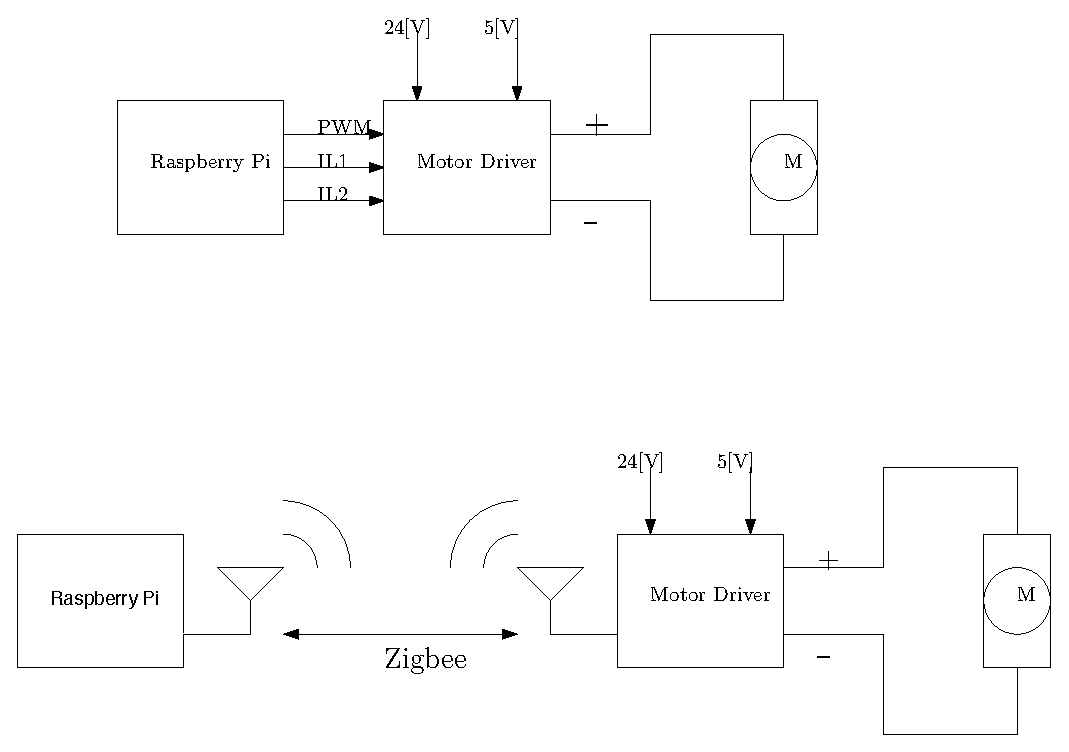
\includegraphics[scale=1]{figs/ipe/RpiMDInterface.eps}
    \caption{Raspberry Pi- Motor Driver Communication}
    \label{fig:RPIMD}
\end{figure}

%subsystem level



\subsection{Specifications}
For our project, we have three main specifications that we will be implemented. The first is that we will be introducing a new supported device within BEMOSS. This device will work with BEMOSS without any configuration changes within the software. The second is to get BEMOSS to work on a new device such as a Raspberry Pi. This is a beneficial portion of our project as it presents the ability to have multiple nodes for different BEMOSS environments. The final specification is to develop an algorithm for BEMOSS energy control. We will determine the amount of energy consumed in an environment without an algorithm employed, how much energy is consumed with BEMOSS running, and how much energy is consumed with the developed algorithm employed within BEMOSS.

\section{Preliminary Work}
After we familiarized ourselves with the architecture and working of BEMOSS, we downloaded and installed the necessary software for the project. To do so, we set up a virtual machine with Ubuntu Linux 16.04. We also did research on what BEMOSS has been used for in the past. This research included who works with the software as well as what it can currently do. 
\subsection{Modelling} \label{sec:model}
We began by creating a model for our motor schematic using Simscape. This model uses a pwm signal coming from a power source that is fed into a H-bridge. This signal is then run through a motor. Power is calculated from this model for later use when designing a neural network algorithm to minimize the cost function.
\begin{figure}
  \centering
  \boxed{\includegraphics{figs/MATLAB/motorModelWithHBridge.png}}
  \caption{Simulink Model of Motor with H Bridge Control}
  \label{fig:motorModelWithHBridge}
\end{figure}
Next we began to create a model for a HVAC system for a house. This model consists of a thermostat, heater and thermal loads. To begin a simple model was used to control the temperature. This controller only checks for the current internal temperature of the house and compares it with the reference temperature point. 
To build on to this model we followed the works of \cite{Reppa2015}\cite{Dhar2018} to develop an adaptive control model for N-number of rooms. 
The control algorithm used for this model is based on a state-space model using the simple system of equations
\begin{equation*}
    \begin{cases} \dot{x} = Ax+Bu \\ y = Cx + Du \end{cases}
\end{equation*}
From \cite{Reppa2015} the system of equations for the single room case is as follows:
\begin{multline*}
    \label{eq:HVAC-Modeling}
    \frac{\mathrm{d}\mathbf{T}^e}{\mathrm{dt}} = 
    \begin{bmatrix}
    \dot{T}_1^e\\
    \dot{T}_2^e    
    \end{bmatrix}
    = 
    \begin{bmatrix}
    -\frac{u_{cc}A_{cc}}{M_{cc}C_v} & \frac{Q_w\rho_w C_{\rho_w}}{M_{cc}C_v}\\
    0 &  -\frac{Q_w\rho_wC_{pw}+U_tA_t}{V_t\rho_wC_{pw}}
    \end{bmatrix}
    \begin{bmatrix}
    T_1^e\\
    T_2^e
    \end{bmatrix}
    +
    \begin{bmatrix}
    \frac{U_{cc}A_{cc}}{M_{cc}C_v}T_{amb} - \frac{Q_w\rho_wC_{pw}}{M_{cc}C_v}T_{wo} \\
    \frac{U_tA_t}{V_t\rho_wC_{pw}}T_{amb} + \frac{Q_w\rho_wC_{pw}}{V_t\rho_wC_{pw}}T_{wo}
    \end{bmatrix}
    +\\
    \begin{bmatrix}
    0 \\
    \frac{15000}{V_t\rho_wC_{pw}}
    \end{bmatrix}
    \chi
    +
    \begin{bmatrix}
    (\frac{\rho_aC_{pa}}{M_{cc}C_v}Q_{a1}-\frac{U_{cc}A_{cc}}{M_{cc}C_v})\\
    0
    \end{bmatrix}    
\end{multline*}

Using the specifications from \cite{Reppa2015} the model becomes:
\begin{equation*}
    \begin{cases} \dot{T_1^e} = -.02815T_1^e + 1.2073T_2^e -0.02815T_{z1} + 0.0005Q_{a1} + 3.932Q_{a1}T_{z1}-3.932Q_{a1}T_{z1}+6.0420\\ \dot{T_2^e} = -0.0007T_2^e + 0.006\chi +.0192 \\ \dot{T}_{z1} = -0.0006T_{z1} - 0.1144T_{z1}Q_{a1} + 0.1144T_1^eQ_{a1} + 0.021\end{cases}
\end{equation*}

This system is controlled by the inputs $Q_{a1}$ and $\chi$. This system is a linear time variant system and therefore needs to be solved using a ordinary differential equation (ode) solver. 

To model this system we chose to use Simulink as it will allow us to easily set up the system and has a built in ode solver and will allow us to more easily connect the house model with the models of our other devices for when we develop a robust energy management system.
%in~\autoref{fig:ackermann}. This model is only used for calculating the steering angle of the mobile robot with pose $\textbf{q}=[q_x, q_y, q_{\theta}]^{T}$ where $(q_x,q_y)$ is the robot's 2D position and $q_{\theta}$ is its orientation with respect to the global coordinate frame. This model will calculate the necessary steering angle to converge toward its current waypoint with location $\textbf{c}=[c_x, c_y]^{T}$ where . In this model the linear velocity is kept at a constant value for simplicity. The steering angle is calculated using

\begin{figure}
    \centering
    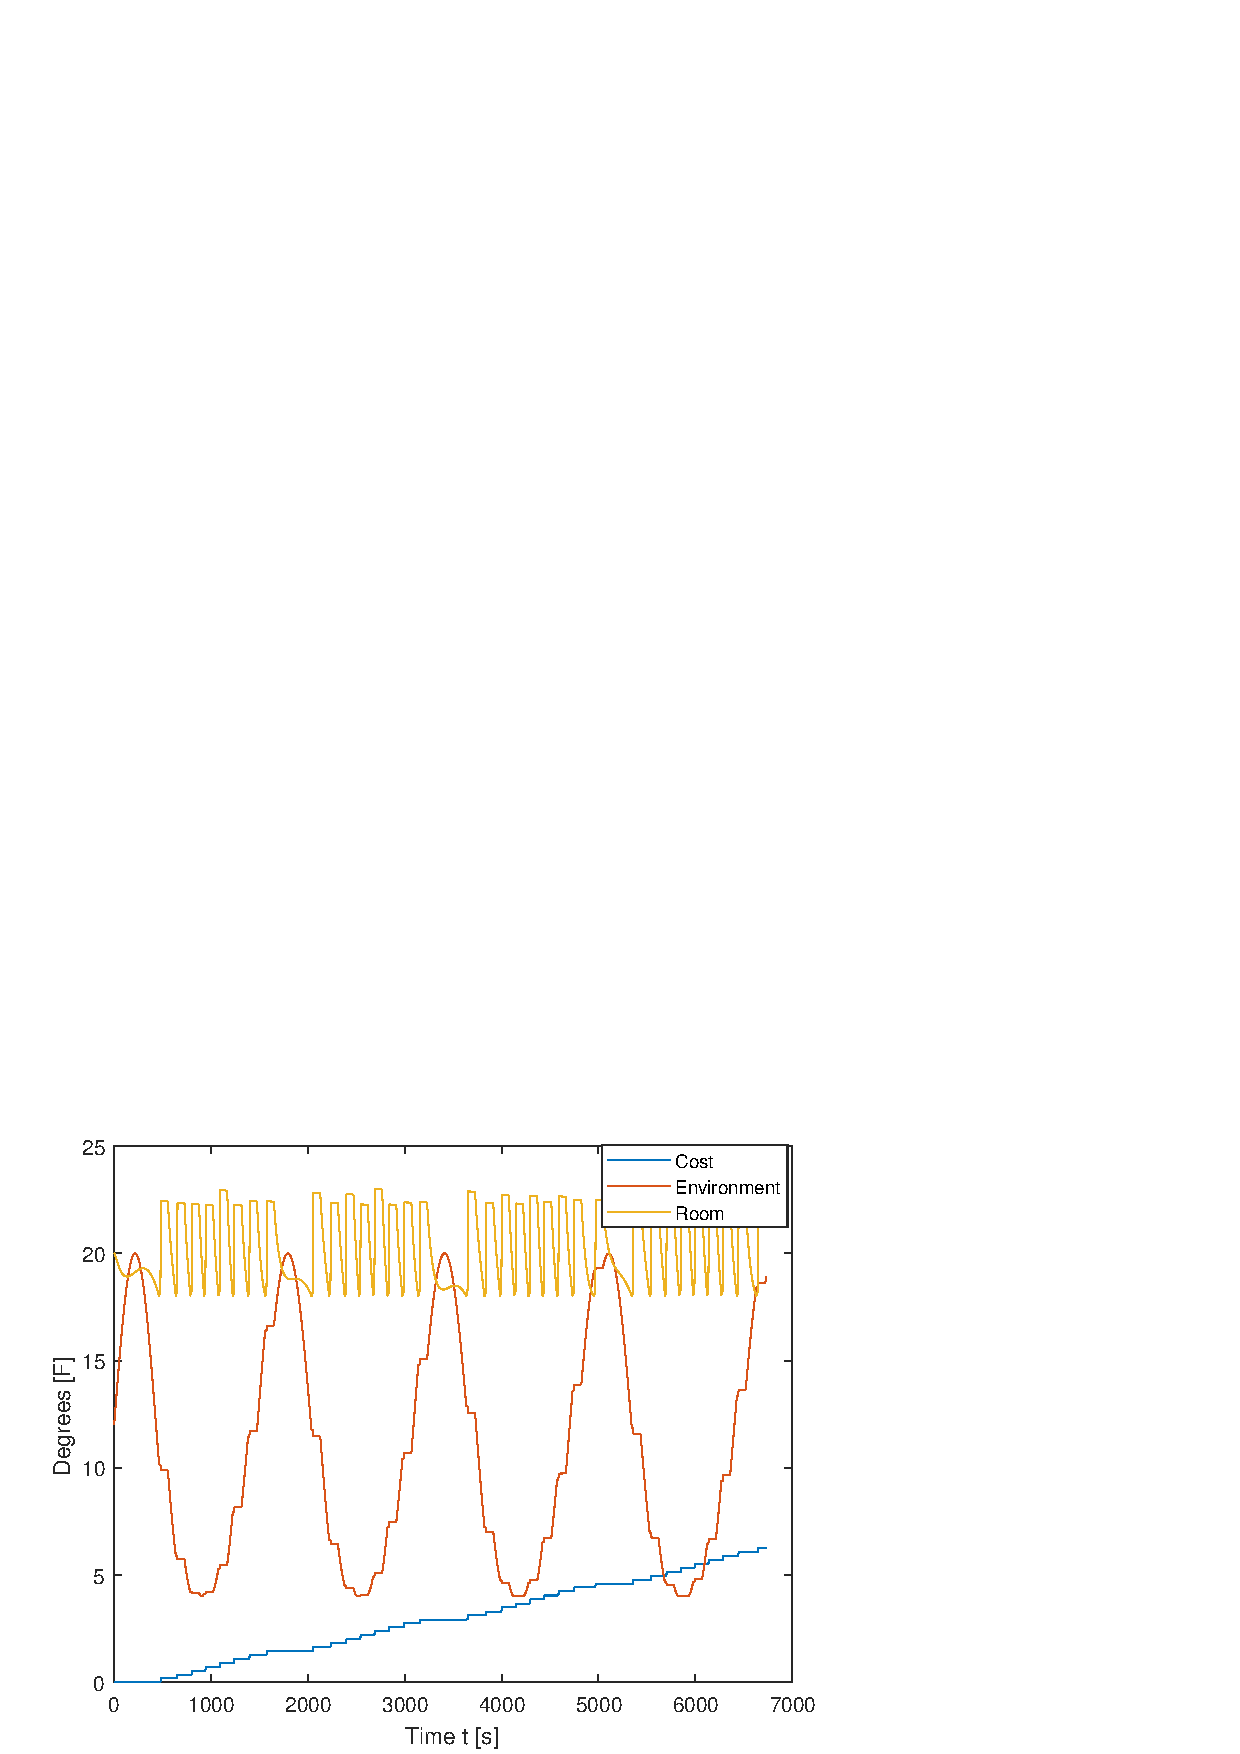
\includegraphics[scale=.85]{figs/MATLAB/houseModel.PNG}
    \caption{Simulink House HVAC Model}
    \label{fig:my_label}
\end{figure}

\subsection{Design} \label{sec:design}
In the fully functioning system, a computer running linux will act as the main BEMOSS control center. From there, a Raspberry Pi 3B microcomputer\footnote{\url{https://raspberrypi.org}} will act as a central node by receiving the commands from the TCP/IP network and transmitting the necessary information to the remote motors over a Zigbee network. In this central node, numerous python scripts will be employed to transmit AT commands to the Xbee network and to employ control algorithms to accurately control and monitor the remote motors. The coordinator XBee will command the remote xBees to toggle 2 of their pins depending on the desired rotation direction of the motor's shaft (as commanded from the BEMOSS control center). These two pins will be connected to a L298N motor driver which will power and switch the polarity of the motor. When either of the remote pins switch high, relays will be activated to supply 5v to the encoder. This power will only be available when the motor is being commanded to turn as to prevent energy waste. The encoder output channels will pass through a TXS0108E logic level converter to transmit the positional data through the remote xBee back to the coordinator XBee. This data will be used to provide a closed loop feedback of the motor's position. The data will be processed on the central node's computer and will influence the precise transmission of the remote motor shut off commands after a certain position has been achieved. \\



%The future work required in the overall design is controlling the mobile robot with the BeagleBone Black microcomputer, and determining the angles of the beacons in relation to the mobile robot. The C program will need expand to a C++ program when implementing the Pioneer 3-DX controller. The Robot Operating System (ROS) is an open source C++ library that simplifies the code needed to control robots. The ROS library should be able to integrate into the existing network interfacing program seamlessly into one network interfacing and control program. To determine the angles of the beacon in relation to the mobile robot, we plan to implement a rotating antenna reflector for the robot mounted XBee in a similar design as~\cite{Hood2011}. This will focus the ping signal in one direction thus resulting in a higher RSSI for beacons in the direction of the reflector and lower RSSI for the beacons in other positions. After taking several RSSI measurements while rotating the reflector, we will be able to determine the angle of a beacon based on its strongest received signal strength.  

\subsection{Experimental Activities} \label{sec:expresults}
Thus far, our work has been oriented towards crafting a useful system by creating a standard functioning product and continually expanding on it's abilities and practicality. Our original design used a Raspberry Pi to send data to a H-Bridge that controlled the rotational direction and speed of rotation of a motor. From there, we expanded the ability of this system by creating a central node that can communicate between numerous remote motors. We did this by incorporating a Zigbee network into our system. We initially used XCTU to initialize the XBee modules and send AT commands through a USB port to a coordinator XBee. From there, the command would be received from remote XBee modules and control a remote motor. After we successfully transmitted commands from XCTU to rotate the motor shaft in either direction, we aimed to make the product more practical. We proceeded to create an interface between the serial port of a Raspberry Pi and the coordinator XBee as to eliminate the need for human interaction in XCTU and allow the ability for additional automation between BEMOSS commands and motor rotation. This Zigbee/ Raspberry Pi interface allows for a single internet connection to control a building's worth of remote blinds and doors. In order to experiment, we created python scripts that send AT commands through the Zigbee network that control the speed of a remote motor and change rotational direction of a remote motor. We are currently expanding on the capabilities of the system by creating a closed-loop feedback system to monitor the position of remote motors. We are currently waiting for an order of relays and logic level converters that will allow for a translation between the 3.3v logic level of XBee modules and the 5v logic level of the encoders and H-Bridges that are employed on each remote motor. When this system is implemented, a command to, say, close curtains will initiate the transmission of a remote AT command to rotate a remote motor in the required direction and monitor the positional data until a certain position is reached. The positional data will only be monitored and transmitted while the motor is activated. This feature is added to prevent unnecessary energy consumption by encoders. 


\begin{figure}
    \centering
    \includegraphics[scale=.1]{figs/ipe/Circuit10_29.JPG}
    \caption{Remote Motor Circuit}
    \label{fig:RRemoteCircuit1}
\end{figure}


We have also been working with already supported BEMOSS devices to research how the software works. We installed BEMOSS on a laptop running Ubuntu 16.04 and controlled a WeMo plug. In order to get BEMOSS to work properly we started on a virtual machine on Bob's laptop. Doing this allowed the server to start but we were not able to find the WeMo plug. The reason we could not find the WeMo plug was because the network settings within a virtual machine are not the same as the network settings on a host computer. The virtual machine attempts to obtain its own ip from a router but the router might not allow this depending on the WiFi card. This was a problem until we were able to obtain a laptop from Mr. Mattus. 
Once we had the laptop we were able to wipe the hard drive to install Linux Ubuntu16.04. This allowed us to work with BEMOSS and the supported devices as intended. We can conclude from this that virtual boxes cause a lot of issues when the connection to the router needs to be final. Bob worked through this for a while and found out that the bridged adapter does not always work. In testing, we discovered that there were a few issues found on the newer versions of Oracle VM VirtualBox and pertaining to the Bridge network. We had hoped that this would solve our problems but after a week or so of testing realized that this was not a possible solution for our issue. (write about what we've done, what didnt work, what you did to make it work, and what we can conclude now that we have it done)   

\begin{center}
    \includegraphics[width=.68\textwidth, keepaspectratio =true]{figs/img/allDevices.png}
    
\end{center}
%\includegraphics[width=.68\textwidth,keepaspectratio=true]{figs/MATLAB/beaconerror}
    %\label{fig:beaconerror}

The device also gives us some data that we will be using in the future. BEMOSS outputs the power usage of each device and allows the user to create a schedule for each device. These features will be utilized in the future to create the neural network algorithm by providing energy cost and by allowing us to reduce the usage of each component by controlling them.
\begin{center}
    \includegraphics[width=.68\textwidth, keepaspectratio=true]{figs/img/plugloadStats.png}
    
\end{center}

\section{Parts List}
Our project consists of some easily accessible components. The linux command center is ran as a parallel operating system on our laptops. On top of a laptop, we utilized 1 Raspberry Pi, 2 XBees, 2 xBee to USB explorers, a L298N motor driver, a Pittman 24v motor,2 breadboards, a TXS0108E logic converter, and 2 3v relays. Most of these parts were acquired in the engineering building for free. We did purchase a few BEMOSS supported plugs to test the functionality of our BEMOSS system before we began exploring new load options and capabilities with our motor. The list of purchased parts can be seen in Table 1. 

\begin{table}
\centering
\begin{tabular}{|c|c|c|}
    \hline
    Part & Price & Quantity \\
    \hline 
    XBee Interface Board & \$5.31 & 1 \\
    \hline
    8 Channel Logic Converter & \$5.99 & 1 \\
    \hline
    $\SI{3.3}{\volt}$ Relay Board & \$11.90 & 1\\
    \hline 
    Buck/ Boost Converter & \$9.99 & 1\\
    \hline 
    WeMo Smart Plug & \$ 27.90 & 2\\
    \hline
\end{tabular}
\caption{List of ordered parts}
\label{tab:ordparts}
\end{table}


%\section{Conclusion}
%\label{sec:conclusion}
%In this paper, we presented a neighboring optimal control law for a mobile robot to track a pre--defined trajectory with its range--limited sensory capabilities. The robot receives signal strength measurement of RF sensors placed on 2-D environment and estimates its states based on the noise sensory model. The robot’s states are partially observed simply because it estimates its position and orientation based on signal strength measurements coming from RF sensors. The proposed controller is the direct consequence of our previously published article but this paper shows how a mobile robot tracks a pre-defined trajectory when RF sensors are placed on 2-D positions and robot receives only signal strength measurements from a subset of RF sensors due its range--limited capabilities.


\bibliographystyle{IEEEtran}
%\bibliography{bibliography/refsSuruzWeb,bibliography/refsRoboticsJournals,bibliography/refsRoboticsConferences,bibliography/refsMultiAgent,bibliography/refsBooksTRTheses}
\bibliography{bib/references.bib}

\end{document} 


%%% Local Variables:
%%% mode: latex
%%% TeX-master: t
%%% End:
